\documentclass[tikz,border=6pt]{standalone}
\usetikzlibrary{arrows.meta,calc,positioning}

\begin{document}
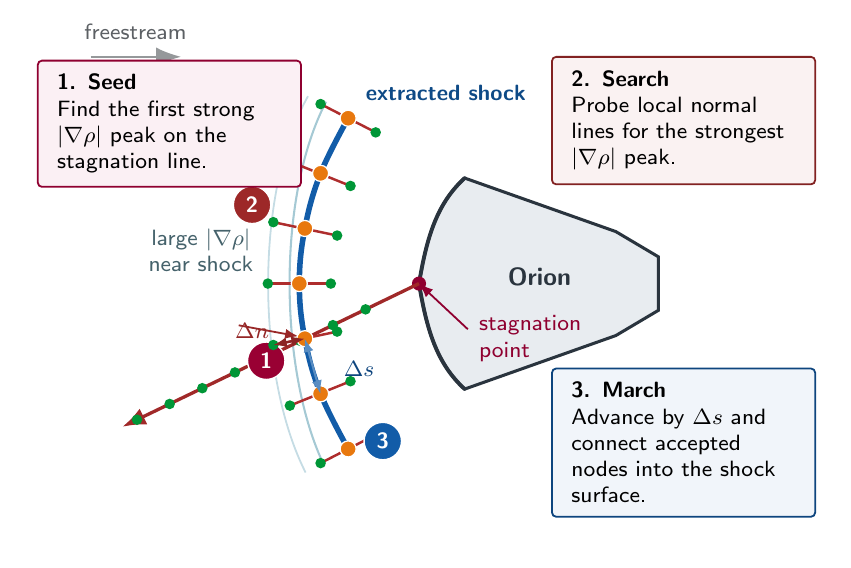
\begin{tikzpicture}[
    x=1cm,
    y=1cm,
    font=\sffamily,
    >=Latex,
    body/.style={draw=bodyline, fill=bodyfill, line width=1.1pt},
    heatshield/.style={draw=bodyline, line width=1.4pt, line cap=round},
    shock/.style={draw=shockblue, line width=2.0pt, line cap=round},
    searchline/.style={draw=searchred, line width=0.9pt, line cap=round},
    initial/.style={draw=searchred!92!black, line width=1.2pt, -{Latex[length=3mm]}},
    sample/.style={circle, fill=samplegreen, inner sep=1.35pt},
    shocknode/.style={circle, fill=nodeorange, draw=white, line width=0.45pt, inner sep=2.05pt},
    callout/.style={
        draw=#1!75!black,
        fill=#1!6,
        rounded corners=1.5pt,
        line width=0.65pt,
        inner xsep=7pt,
        inner ysep=5pt,
        text width=2.85cm,
        align=left,
        font=\sffamily\footnotesize
    },
    tag/.style={
        circle,
        fill=#1,
        draw=white,
        line width=0.5pt,
        text=white,
        font=\sffamily\bfseries\footnotesize,
        inner sep=2.3pt
    }
]

\definecolor{shockblue}{RGB}{18,92,168}
\definecolor{searchred}{RGB}{174,45,45}
\definecolor{nodeorange}{RGB}{232,120,14}
\definecolor{samplegreen}{RGB}{0,150,55}
\definecolor{bodyfill}{RGB}{232,236,240}
\definecolor{bodyline}{RGB}{42,52,62}
\definecolor{notegrey}{RGB}{92,96,100}
\definecolor{fieldline}{RGB}{126,178,194}

\path[use as bounding box] (-5.15,-3.25) rectangle (4.95,3.25);

\coordinate (stag) at (-0.18,0.00);
\coordinate (farstart) at (-3.95,-1.82);
\coordinate (seed) at (-1.63,-0.70);

% Freestream direction.
\draw[-{Latex[length=3.2mm]}, line width=0.85pt, notegrey!65]
    (-4.35,2.88) -- (-3.20,2.88);
\node[anchor=south, text=notegrey, font=\sffamily\footnotesize]
    at (-3.78,2.98) {freestream};

% Orion capsule cross-section: curved heat shield plus conical backshell.
\path[body]
    (stag)
    .. controls (-0.08,0.60) and (0.05,1.02) .. (0.40,1.34)
    -- (2.32,0.66)
    -- (2.86,0.34)
    -- (2.86,-0.34)
    -- (2.32,-0.66)
    -- (0.40,-1.34)
    .. controls (0.05,-1.02) and (-0.08,-0.60) .. (stag)
    -- cycle;
\draw[heatshield]
    (0.40,-1.34)
    .. controls (0.05,-1.02) and (-0.08,-0.60) .. (stag)
    .. controls (-0.08,0.60) and (0.05,1.02) .. (0.40,1.34);
\node[text=bodyline, font=\sffamily\bfseries\small] at (1.35,0.08) {Orion};
\node[circle, fill=purple!75!black, inner sep=1.8pt] at (stag) {};
\draw[purple!75!black, line width=0.65pt, -{Latex[length=1.8mm]}]
    (0.44,-0.58) -- (stag);
\node[anchor=west, align=left, text=purple!75!black, font=\sffamily\footnotesize]
    at (0.46,-0.70) {stagnation\\point};

% A few subdued density-gradient contours. No halo around the shock.
\draw[fieldline!70, line width=0.75pt]
    (-1.38,-2.32) .. controls (-1.95,-1.15) and (-2.00,1.08) .. (-1.36,2.31);
\draw[fieldline!45, line width=0.65pt]
    (-1.62,-2.40) .. controls (-2.24,-1.18) and (-2.28,1.14) .. (-1.59,2.38);
\node[text=fieldline!55!black, font=\sffamily\footnotesize, align=center]
    at (-2.95,0.42) {large $|\nabla\rho|$\\near shock};

% Initial stagnation-line search. The seed node lies on this line.
\draw[initial] (stag) -- (farstart);
\foreach \t in {0.18,0.29,0.40,0.51,0.62,0.73,0.84,0.95} {
    \node[sample] at ($(stag)!\t!(farstart)$) {};
}
\draw[searchred!88!black, line width=0.65pt, -{Latex[length=1.7mm]}]
    (-2.47,-0.53) -- ($(seed)+(-0.08,0.03)$);
\node[tag=purple!80!black] at (-2.12,-0.98) {1};

% Normal search rays. Center points match the shock nodes below.
\foreach \px/\py/\ax/\ay/\bx/\by in {
    -1.08/-2.10/-1.43/-2.28/-0.73/-1.92,
    -1.43/-1.40/-1.82/-1.55/-1.05/-1.24,
    -1.63/-0.70/-2.03/-0.78/-1.22/-0.61,
    -1.70/0.00/-2.10/0.00/-1.30/0.00,
    -1.63/0.70/-2.03/0.78/-1.22/0.61,
    -1.43/1.40/-1.82/1.55/-1.05/1.24,
    -1.08/2.10/-1.43/2.28/-0.73/1.92
} {
    \draw[searchline] (\ax,\ay) -- (\bx,\by);
    \node[sample] at (\ax,\ay) {};
    \node[sample] at (\bx,\by) {};
}
\node[tag=searchred!90!black] at (-2.30,1.00) {2};

% Extracted shock curve drawn through the exact shock-node coordinates.
\draw[shock]
    plot[smooth, tension=0.65] coordinates {
        (-1.08,-2.10)
        (-1.43,-1.40)
        (-1.63,-0.70)
        (-1.70,0.00)
        (-1.63,0.70)
        (-1.43,1.40)
        (-1.08,2.10)
    };
\foreach \x/\y in {
    -1.08/-2.10,
    -1.43/-1.40,
    -1.63/-0.70,
    -1.70/0.00,
    -1.63/0.70,
    -1.43/1.40,
    -1.08/2.10
} {
    \node[shocknode] at (\x,\y) {};
}
\node[tag=shockblue] at (-0.64,-2.00) {3};
\node[anchor=west, text=shockblue!80!black, font=\sffamily\bfseries\footnotesize]
    at (-0.98,2.42) {extracted shock};

% Local spacing annotations.
\draw[shockblue!70, line width=0.75pt, {Latex[length=1.7mm]}-{Latex[length=1.7mm]}]
    (-1.43,-1.40) -- (-1.63,-0.70);
\node[anchor=west, text=shockblue!75!black, font=\sffamily\footnotesize]
    at (-1.26,-1.08) {$\Delta s$};
\draw[searchred!80!black, line width=0.75pt, {Latex[length=1.7mm]}-{Latex[length=1.7mm]}]
    (-2.03,-0.78) -- (-1.63,-0.70);
\node[anchor=south east, text=searchred!85!black, font=\sffamily\footnotesize]
    at (-1.96,-0.82) {$\Delta n$};

% Three step callouts, kept outside the geometry.
\node[callout=purple] (stepone) at (-3.35,2.03)
    {\textbf{1. Seed}\\Find the first strong $|\nabla\rho|$ peak on the stagnation line.};

\node[callout=searchred] (steptwo) at (3.18,2.07)
    {\textbf{2. Search}\\Probe local normal lines for the strongest $|\nabla\rho|$ peak.};

\node[callout=shockblue] (stepthree) at (3.18,-2.02)
    {\textbf{3. March}\\Advance by $\Delta s$ and connect accepted nodes into the shock surface.};

\end{tikzpicture}
\end{document}
